\documentclass{article}
\usepackage[utf8]{inputenc}
\usepackage{array}
\usepackage{wrapfig}
\usepackage{multirow}
\usepackage{tabu}
\usepackage{graphicx}
\usepackage{float}

\title{Report}
\author{Koray Can Yurtseven}
\date{24.03.2018}

\begin{document}

\maketitle

\section{PART 1}
\subsection{Network 1 Graph}
\begin{figure}[H]
  \caption{Arch1 Sigmoid}
  \centering
  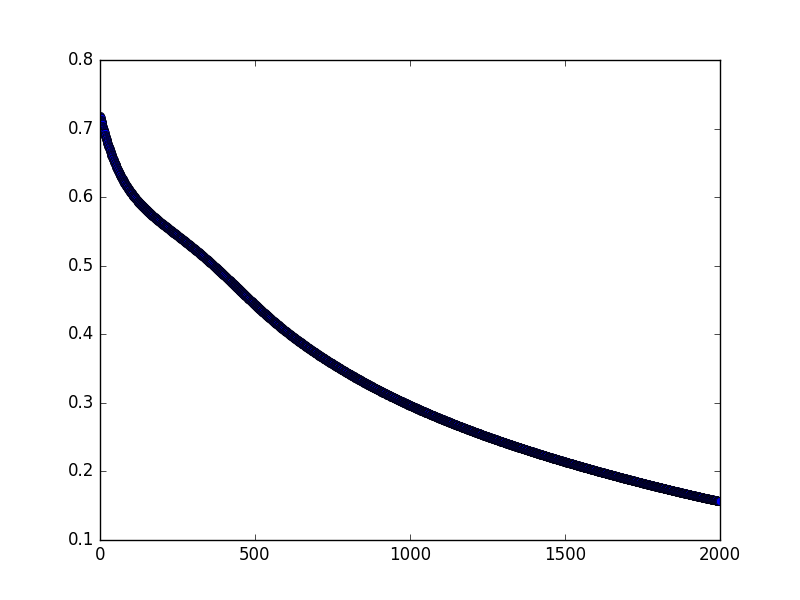
\includegraphics[width=0.8\textwidth]{arch1sigmoid}
\end{figure}
\begin{figure}[H]
  \caption{Arch1 Tanh}
  \centering
  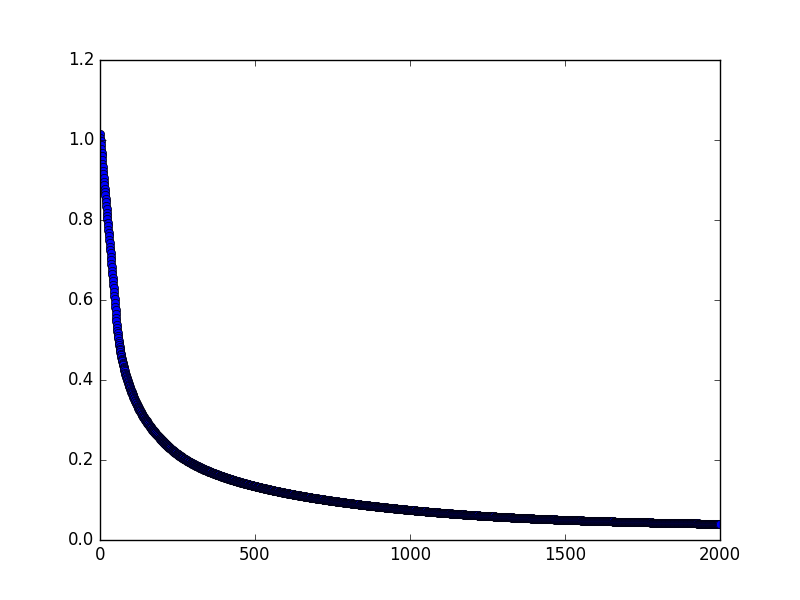
\includegraphics[width=0.8\textwidth]{arch1tanh}
\end{figure}
\begin{figure}[H]
  \caption{Arch1 Relu}
  \centering
  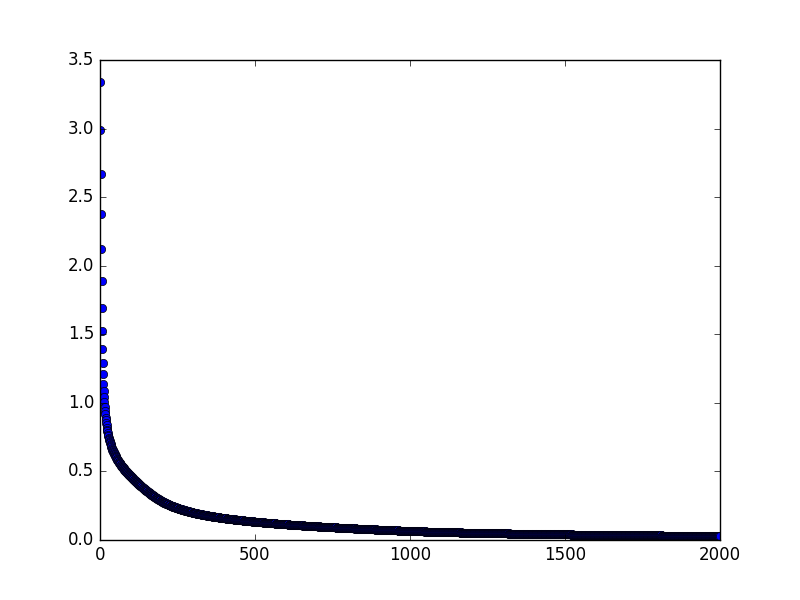
\includegraphics[width=0.8\textwidth]{arch1relu}
\end{figure}
\subsection{Network 2 Graph}
\begin{figure}[H]
  \caption{Arch2 Sigmoid}
  \centering
  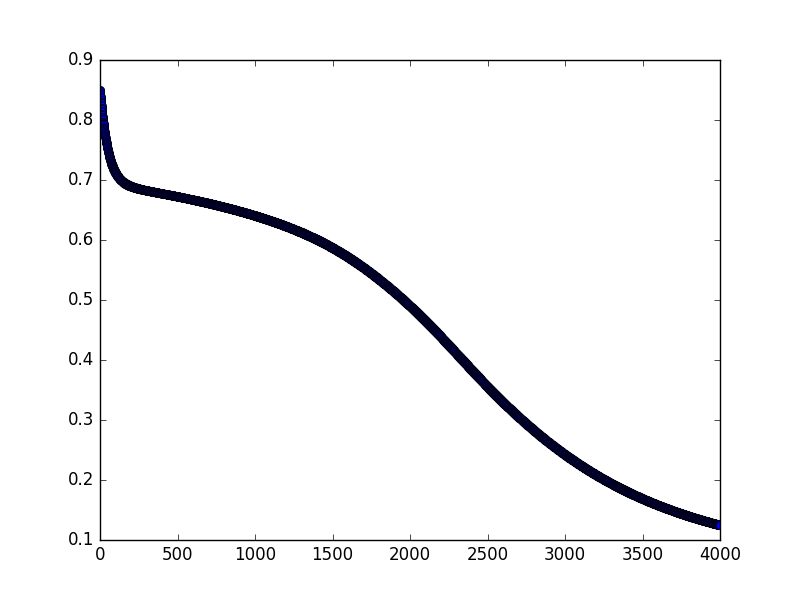
\includegraphics[width=0.8\textwidth]{arch2sigmoid}
\end{figure}
\begin{figure}[H]
  \caption{Arch2 Tanh}
  \centering
  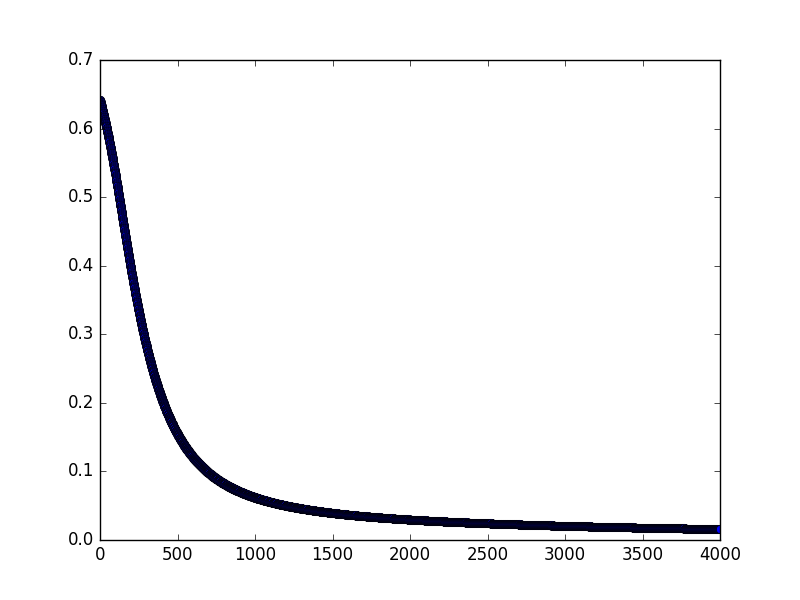
\includegraphics[width=0.8\textwidth]{arch2tanh}
\end{figure}
\begin{figure}[H]
  \caption{Arch2 Relu}
  \centering
  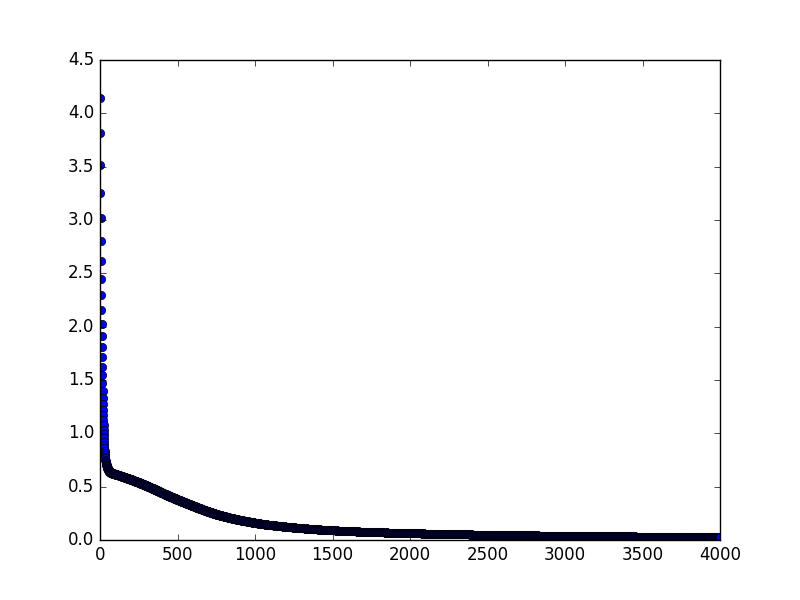
\includegraphics[width=0.8\textwidth]{arch2relu}
\end{figure}
\subsection{Network 3 Graph}
\begin{figure}[H]
  \caption{Arch3 Sigmoid}
  \centering
  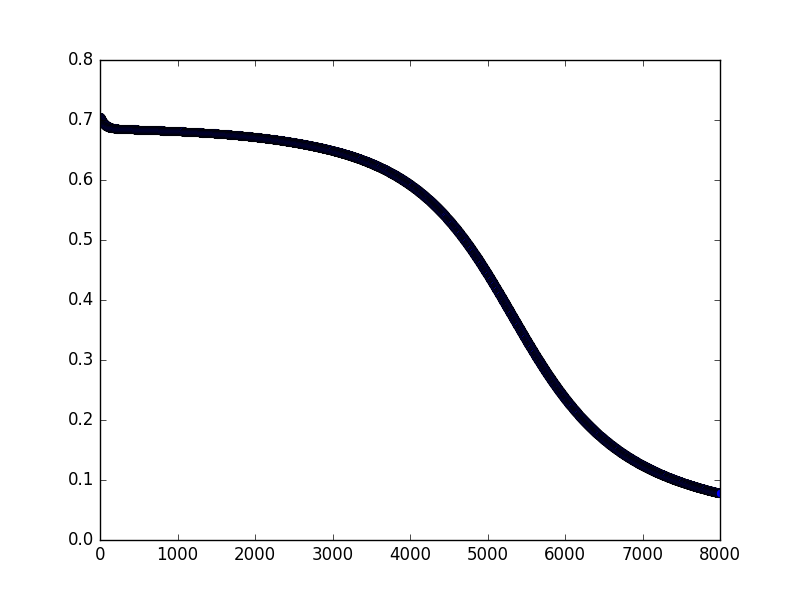
\includegraphics[width=0.8\textwidth]{arch3sigmoid}
\end{figure}
\begin{figure}[H]
  \caption{Arch3 Tanh}
  \centering
  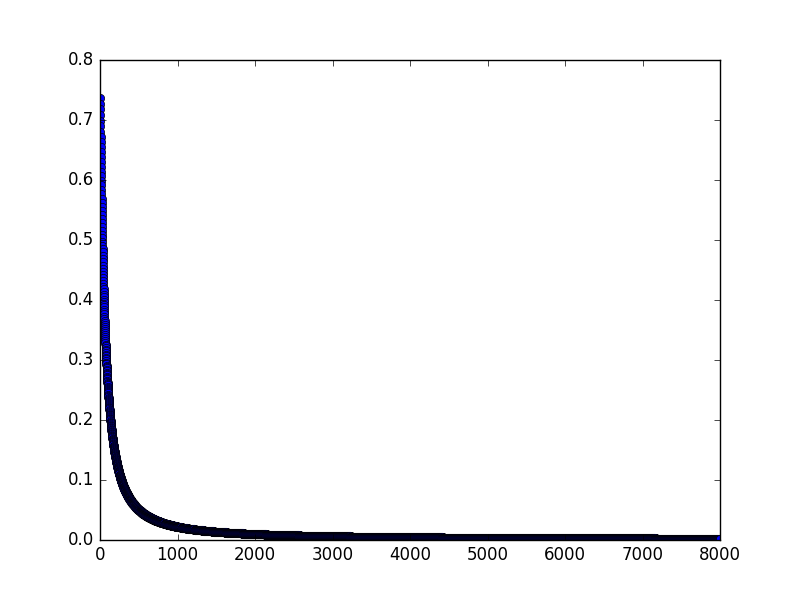
\includegraphics[width=0.8\textwidth]{arch3tanh}
\end{figure}
\begin{figure}[H]
  \caption{Arch3 Relu}
  \centering
  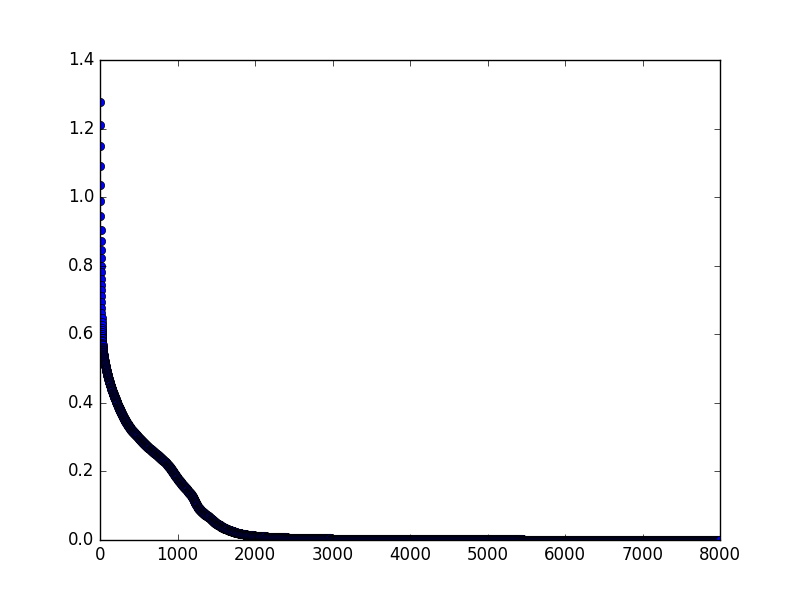
\includegraphics[width=0.8\textwidth]{arch3relu}
\end{figure}

\subsection{Final Accuracy For Each Network}

\begin{table}[H]
\centering
\caption{Final Accuracy For Each Network}
\begin{tabular}{|l|l|l|l|l}
\cline{1-4}
         & Sigmoid    & Tanh      & Relu      &  \\ \cline{1-4}
Network1 & 0.989083   & 0.9934498 & 0.9956332 &  \\ \cline{1-4}
Network2 & 0.99126637 & 1.0       & 1.0       &  \\ \cline{1-4}
Network3 & 0.9934498  & 1.0       & 0.9978166 &  \\ \cline{1-4}
\end{tabular}
\end{table}

\subsection{Hyperparameter Optimization}
\subsubsection{Optimization}
Explain how you have used training data to optimize your parameters, your optimization criteria. Fill the following table based on the given parameters and value acquired from optimization criteria. 
\begin{table}[H]
    \resizebox{\columnwidth}{!}{%
    \centering
    \begin{tabular}{|c|c|c|c|c|c|c|c|c|c|c|}
    \hline
    \multirow{2}{5em}{Layer Activations} & \multicolumn{10}{c|}{Learning Rate} \\
        & 0.01 & 0.02 & 0.03 & 0.04 & 0.05 & 0.06 & 0.07 & 0.08 & 0.09 & 0.1 \\
        \hline \hline
        SSS & val & val & val & val & val & val & val & val & val & val \\
        \hline
        SST & val & val & val & val & val & val & val & val & val & val \\
        \hline
        SSR & val & val & val & val & val & val & val & val & val & val \\
        \hline
        STS & val & val & val & val & val & val & val & val & val & val \\
        \hline
        STT & val & val & val & val & val & val & val & val & val & val \\
        \hline
        STR & val & val & val & val & val & val & val & val & val & val \\
        \hline
        SRS & val & val & val & val & val & val & val & val & val & val \\
        \hline
        SRT & val & val & val & val & val & val & val & val & val & val \\
        \hline
        SRR & val & val & val & val & val & val & val & val & val & val \\
        \hline
        TSS & val & val & val & val & val & val & val & val & val & val \\
        \hline
        TST & val & val & val & val & val & val & val & val & val & val \\
        \hline
        TSR & val & val & val & val & val & val & val & val & val & val \\
        \hline
        TTS & val & val & val & val & val & val & val & val & val & val \\
        \hline
        TTT & val & val & val & val & val & val & val & val & val & val \\
        \hline
        TTR & val & val & val & val & val & val & val & val & val & val \\
        \hline
        TRS & val & val & val & val & val & val & val & val & val & val \\
        \hline
        TRT & val & val & val & val & val & val & val & val & val & val \\
        \hline
        TRR & val & val & val & val & val & val & val & val & val & val \\
        \hline
        RSS & val & val & val & val & val & val & val & val & val & val \\
        \hline
        RST & val & val & val & val & val & val & val & val & val & val \\
        \hline
        RSR & val & val & val & val & val & val & val & val & val & val \\
        \hline
        RTS & val & val & val & val & val & val & val & val & val & val \\
        \hline
        RTT & val & val & val & val & val & val & val & val & val & val \\
        \hline
        RTR & val & val & val & val & val & val & val & val & val & val \\
        \hline
        RRS & val & val & val & val & val & val & val & val & val & val \\
        \hline
        RRT & val & val & val & val & val & val & val & val & val & val \\
        \hline
        RRR & val & val & val & val & val & val & val & val & val & val \\
        \hline
        
\end{tabular}%
}
\end{table}

where S is \verb|sigmoid|, T is \verb|tanh| and R is \verb|relu| activation function. Highlight the values with the best result.
\subsubsection{Training and Test}
Draw the training graph for the best network and report the final classification accuracy here.
\section{PART 2}
Explain your network in detail. Draw the final trainingloss/epoch graph and report your final classification accuracy.
\end{document}
